% Copyright (c) 2016 Ongun Kanat <ongun.kanat@gmail.com>
% This document is a free software licensed under MIT license.
% For redistribution details look at COPYING file.

% 12pt and ISO A4 paper with title page add notitlepage for otherwise
\documentclass[a4paper, 12pt, titlepage]{article}

% 2cm margin from all sides
\usepackage[a4paper,margin=2cm]{geometry}

% Use American English for dates etc.
\usepackage[american]{babel}
% If document is in Turkish then use
% \usepackage[turkish]{babel}
% or for both
% \usepackage[turkish,american]{babel}

% Indent at section beginnings
% \usepackage{indentfirst} % look at below for reverse
% Paragraph spacings set parindent to 0
\setlength{\parindent}{0pt}
\setlength{\parskip}{12pt}

% utf-8 support
\usepackage[utf8]{inputenc}

% Graphics for PDFTeX
\usepackage[pdftex]{graphicx}

% Figure placement
\usepackage{float}

% An enumeration package for flexible enumeration
\usepackage{enumitem}

% Courier monospace font
\usepackage{courier}

% Links, both local and external
\usepackage{hyperref}
\hypersetup{
	unicode=true,
	colorlinks=true,
	urlcolor=blue,
	citecolor=black,
	menucolor=black,
	linkcolor=black
}

% Figure captions are bold
\usepackage[labelfont=bf]{caption}

% Pseudocode
\usepackage{algorithmicx}
\usepackage{algpseudocode}
\usepackage{algorithm}

% Syntax highlighting simple
\usepackage{listings}
\lstset{basicstyle=\ttfamily,frame=lines,tabsize=4}
\renewcommand{\lstlistingname}{Code}

% Syntax higlighting (advanced)
%\usepackage{minted}

% Title, author and date info
\title{My Glorious Report}
\author{Hasan Fatih Durkaya \\ 150200074}
\date{December 2, 2022}

\begin{document}
% Fix Turkish fix hypenation
%\shorthandoff{=}

% For a generic title page one can use standard \maketitle command
% It will use the title info above
% \maketitle

% The title page can be made by hand as below
\begin{titlepage}
	\begin{center}
		\large{Istanbul Technical University \\ Faculty of Computer and Informatics \\ Computer Engineering Department} \\
		\vspace{150pt}
		\Large{BLG 335E \\ Analysis of Algorithms I Homework 2 }  \\
		\vspace{30pt}

		\large{Hasan Fatih Durkaya - 150200074} \\
		\vspace{\fill} % Fill out until the page end
		\large{December 2\textsuperscript{nd}, 2022}
	\end{center}
\end{titlepage}
\pagenumbering{roman}
\newpage
\tableofcontents
\newpage

\pagenumbering{arabic}
\section{Introduction}
In this homework, we are asked to create a system to store and organize data according to expectations. For this purpose, we have to follow some rules to manage data. This an important topic becausersituationts like this homework that includeing tens of thousands of data maybe millions are everywhere nowadays and storing it efficiently is an important problem .

\section{Data Structures}
    In this homework I have used heap and vectors. Heap data structure is used to build a heap then apply heap sort on that because of it's lower complexity when we compare it to other sorting algorithms. Vectors are used for general storing purposes it's dynamic structure is an important properity.

\subsection{Heap}
    Heap is a special tree-based data structure which is nearly a complete tree that has to satisfy one critical condition: Heap Properity. For instance, a max-heap for any node parent must be greater or equal to it's child. In a min-heap this case is reversed parent must be lower or equal to it's child's key value. The first node is called "root". We use a tree-based approach but we store heaps in arrays or vectors and there is relation between parent - child indexes. If we know the index of a parent we can acces to it's child without special getter function.One of the most important topics about heaps is heap sort. Heap sort is an sorting algorithm which uses heap data structure and has a time complexity O(nlogn) in all cases. This is important because it gives us the stability that we seek. 

        

\subsection{Vectors}
    Vectors are nearly the same with dynamic arrays with ability to manage it's size when an element is inserted or deleted. I have used vectors to store 2 different values: expected functions that we are looking for like median, firstq  (wanted values) and all the dataset that contain gap,gi,grp and v (dataset).

\usepackage{\textbf{Vectors used}} 
\begin{lstlisting}[language=C++]
vector<string> wanted_values;      
vector<float> dataset;            
\end{lstlisting}

Wanted values is string because we are not going to make an operation on them we will check just what are those on the other hand dataset is float because we have to make some operations with precision.

\section{Basics of Implementation}
    
    In this part, I am going to cover critical points of implementation. We are looking for efficiency and lower computational cost, in order to achieve that there are some key points.
    
\usepackage{\textbf{Adding}}
\begin{lstlisting}[language=C++]
    if(temp == "add"){
        if(expected_temp == "gap"){
            if(counter == 0){
                    getline(fin, first_date, ',');
                    getline(fin, first_hour, ',');
\end{lstlisting}

    For example, when we are adding we don't want to store the values that we are not interested in. If we are looking for mean of gap we don't have store grp or gi in vector . It will cause huge amount of memory usage , to overcome this memory efficiency problem I have create an if-else structure and the type of parameter is gap we only take the first elements of the input stream after the dates. On the other hand inside if loop checks the is it the first time that we are getting inputs to get the first date and first hour to print.In this case we are just ignoring the other 3 types (grp, gi,v) of parameters because we don't need them at all.



\usepackage{\textbf{Printing}}
\begin{lstlisting}[language=C++]
    for(int i = 0; i < size; i++){
        if(wanted_values[i] == "mean"){
            myfile << get_mean(dataset, counter);
                    //cout<<get_mean(dataset, counter);
                    if(func_count < size){
                        myfile << ",";
                        func_count++;
                    }
\end{lstlisting}

    Another key point is we are not calling the functions if we are adding we are calling them only if we are printing something out because if we call them in every input that might cause memory problems. We are checking wanted values vector's elements in a closed loop to call the proper function.

\newpage
\section{Functions}

\subsection{Get Mean}
    Function to calculate mean, this is a basic mean function. Taking input parameters the dataset and a counter to get the size. Basically adding all the values up and dividing result by size.

\begin{algorithm}[H]
	\caption{The calculating mean of an vector}
	\label{algo:dfs}
	\begin{algorithmic}

	\Function{getMean}{$dataset$, $counter$}
		
            \State\ $sum$
            \State\ $mean$ 

			      \For{\texttt{n < counter}}
                    \State \texttt{n = n + dataset[n]}
                    \EndFor
            \State \texttt{mean = sum/counter}
		\State \Return $ mean $
	\EndFunction
	\end{algorithmic}
\end{algorithm}

\usepackage{\textbf{Code for Get Mean}}
\begin{lstlisting}[language=C++]
float get_mean(vector<float> datas, int counter){         
    float mean;
    float sum;

    for(int i = 0; i < counter; i++)
        sum = sum + datas[i];       

    mean = (sum / counter);
    return mean;
}
\end{lstlisting}
Time complexity of this function is O(n) because we are linearly iterating the vector once and since there is only n elements complexity is O(n)

\newpage

\subsection{Get Min}
    Function to calculate minimum, this is a basic min function. Taking input parameters the dataset, is sorted flag and a counter to get the size. Basically if is sorted flag is 0 which means dataset is not sorted we use linear search to get the minimum value. On the other hand if flag is 1 it means dataset is already sorted so we just have to get the first value because it is the minimum

\begin{algorithm}[H]
	\caption{The calculating mean of a vector}
	\label{algo:dfs}
	\begin{algorithmic}

	\Function{getMin}{$dataset$, $counter$,$isSorted$}
		
            \State\ $sum$
            \State\ $min = dataset[0]$ 

            \If{isSorted == 1}
                \State \Return $ min $
            \EndIf
		\For{\texttt{n < counter}}
                \If{\texttt{min > dataset[n]}}
                    \State $ min = dataset[n] $
                \EndIf
            \EndFor
		\State \Return $ min $
	\EndFunction
	\end{algorithmic}
\end{algorithm}


\usepackage{\textbf{Code for Get Min}}
\begin{lstlisting}[language=C++]
float get_min(vector<float> datas, float counter, int is_sorted){           
        
    float min = datas[0];

    if(is_sorted == 1){                        
        return min;
    }
    else{
        for(int i = 0; i < counter; i++){
            if(min > datas[i])
                min = datas[i];
        }
        return min;
    }    
}
\end{lstlisting}
Time complexity of this function is O(n) if the dataset is not sorted because we use linear search but if it is sorted complexity is O(1) since we simply return first element.
\newpage

\subsection{Get Max}

    Function to calculate maximum, this is a basic max function. Taking input parameters the dataset, is sorted flag and a counter to get the size. Basically if is sorted flag is 0 which means dataset is not sorted we use linear search to get the maximum value. On the other hand if flag is 1 it means dataset is already sorted so we just have to get the last value because it is the maximum.

\begin{algorithm}[H]
	\caption{The calculating max of a vector}
	\label{algo:dfs}
	\begin{algorithmic}

	\Function{getMax}{$dataset$, $counter$,$isSorted$}
		
            \State\ $sum$
            \State\ $max = dataset[0]$ 

            \If{isSorted == 1}
                \State \Return $ dataset[counter] $
            \EndIf
		\For{\texttt{n < counter}}
                \If{\texttt{max < dataset[n]}}
                    \State $ max = dataset[n] $
                \EndIf
            \EndFor
		\State \Return $ max $
	\EndFunction
	\end{algorithmic}
\end{algorithm}

    
\usepackage{\textbf{Codeode for Get Max}}
\begin{lstlisting}[language=C++]
float get_max(vector<float>datas, double counter, int is_sorted){       
    
    float max = datas[0];

    if(is_sorted == 1){                     
        return datas[counter];
    }
    else{
        
        for(int i = 0; i < counter; i++){
            
            if(max < datas[i]){
                max = datas[i];
            }
        }
        return max;
    }
}
\end{lstlisting}
Time complexity of this function is O(n) if the dataset is not sorted because we use linear search but if it is sorted complexity is O(1) since we simply return last element.

\subsection{Get Standard Deviation}

    Function to calculate Standard Deviation. Taking input parameters the dataset and a counter to get the size. First we are getting the mean with get mean function then iterating over the dataset and subtracting mean from the value after that taking the square of the result and adding them up . At last dividing it to size minus 1 and taking the root.

\begin{algorithm}[H]
	\caption{The calculating standard deviation of a vector}
	\label{algo:dfs}
	\begin{algorithmic}

	\Function{getStd}{$dataset$, $counter$}
		
            \State\ $std$
            \State $mean = $\Call{getMean}{$ dataset $,$ counter $} 


		\For{\texttt{n < counter}}
                \If{\texttt{max < dataset[n]}}
                    \State $ std += (dataset[n]-mean)*(dataset[n]-mean) $
                \EndIf
            \EndFor
		\State \Return $ (std/counter-1)^(1/2) $
	\EndFunction
	\end{algorithmic}
\end{algorithm}
    
\usepackage{\textbf{Code for Get Standard Deviation}}
\begin{lstlisting}[language=C++]
float get_std(vector<float> datas, float counter){          
    double mean = get_mean(datas,counter);
    double std;

    for(int i = 0; i < counter; i++){
        std += (datas[i] - mean) * (datas[i] - mean);
    }
    
    return sqrt(std/(counter-1));
}
\end{lstlisting}
Time complexity of this function is O(n) because again we are just linearly iterating over a vector. 

\newpage

\subsection{Get Median}

    Function to calculate Median. Taking input parameters dataset and counter to get the size. First of all to get the median we should sort the vector. After the sorting operation we check if the size is odd we take the middle element if it is even, we are calculating the mean of middle two elements.Sorting algorithm is all there is and heapSort will be covered later parts.
\begin{algorithm}[H]
	\caption{The calculating median of a vector}
	\label{algo:dfs}
	\begin{algorithmic}

	\Function{getMedian}{$dataset$, $counter$}
		
            \State \Call{heapSort}{$ dataset $,$ counter $} 

                \If{\texttt{size mod 2 == 0}}
                    \State \Return $ (dataset[counter/2] + dataset[counter/2-1])/2 $
                \EndIf
                \If{\texttt{size mod 2 == 1}}
		          \State \Return $ dataset[counter/2] $
                \EndIf
	\EndFunction
	\end{algorithmic}
\end{algorithm}
    
\usepackage{\textbf{Code for Get Median}}
\begin{lstlisting}[language=C++]
float get_median(vector<float>datas, int size){         
    
    heapSort(datas,size);                               
    
    if(size % 2 == 0)                                   
        return ((datas[size/2] + datas[size/2-1])/2);
    else{
        return datas[size/2];
    }
}
\end{lstlisting}
Time complexity of this function is same as time complexity of heapSort which is nlogn , analysis of this system will be covered in later parts.

\newpage

\subsection{Get First Quartile}

    Function to calculate first quartile. First quartile is the value under which 25 percent of the data points are found , when they are sorted in increasing order. It is an important feature understand the meaning of data. 
\begin{algorithm}[H]
	\caption{The calculating first quartile of a vector}
	\label{algo:dfs}
	\begin{algorithmic}

	\Function{getfirstq}{$dataset$, $counter$}
		
            \State\Call{heapSort}{$ dataset $,$ counter $}

            \State $step$\ {$ = 100/counter-1$} 
            \State $left$\ {$ = 25/step$}
            \State $right$\ {$ = left + 1$}

            \State $lcoef$\ {$ = 1 - (25 - left * step) / step$} 
            \State $rcoef$\ {$ = 1 - lcoef$} 

            \State $quartile$\ {$ = (dataset[left] * lcoef) + (dataset[right_bound] * rcoef)$} 

	\EndFunction
	\end{algorithmic}
\end{algorithm}
    
\usepackage{\textbf{Code for Get First Quartile}}
\begin{lstlisting}[language=C++]
float get_first_quartile(vector<float>datas, int size){    

    heapSort(datas,size);                                 

    double step = 100/double(size - 1);                     
    int left_bound = (25/step);                             

    int right_bound = (left_bound + 1);                    

    float l_coefficent = 1 - ((25 - left_bound * step) / (float)step);     
    float r_coefficent = 1 - l_coefficent;                                 

    float quartile = datas[left_bound]*l_coefficent+datas[right_bound]*r_coefficent;  

    return quartile;
}
\end{lstlisting}
Time complexity of this function is same as time complexity of heapSort because of other parts of this function is constant time.

\newpage

\subsection{Get Third Quartile}

    Function to calculate third quartile. Third quartile is the value higher which 75 percent of the data points are found , when they are sorted in increasing order. It is an important feature understand the meaning of data. 
\begin{algorithm}[H]
	\caption{The calculating third quartile of a vector}
	\label{algo:dfs}
	\begin{algorithmic}

	\Function{getthirdq}{$dataset$, $counter$}
		
            \State\Call{heapSort}{$ dataset $,$ counter $}

            \State $step$\ {$ = 100/counter-1$} 
            \State $left$\ {$ = 75/step$}
            \State $right$\ {$ = left + 1$}

            \State $lcoef$\ {$ = 1 - (75 - left * step) / step$} 
            \State $rcoef$\ {$ = 1 - lcoef$} 

            \State $quartile$\ {$ = (dataset[left] * lcoef) + (dataset[right_bound] * rcoef)$} 

	\EndFunction
	\end{algorithmic}
\end{algorithm}
    
\usepackage{\textbf{Code for Get Third Quartile}}
\begin{lstlisting}[language=C++]
float get_third_quartile(vector<float>datas, int size){             

    heapSort(datas,size);                                          

    double step = 100/double(size - 1);                             
    int left = (75/step);                                     

    int right = (left + 1);                             

    float l_coef = 1 - ((75 - left_bound * step) / (float)step);      
    float r_coef = 1 - l_coefficent;                                  

    float quartile = (datas[left]*l_coef)+(datas[right]*r_coef);  

    return quartile;
}
\end{lstlisting}
Time complexity of this function is same as time complexity of heapSort because of other parts of this function is constant time.

\newpage

\subsection{Heapify}

    Function to build heap data structure which satisfies heap properity. Heap structure is the essential part of heapSort.
\begin{algorithm}[H]
	\caption{Heapify}
	\label{algo:dfs}
	\begin{algorithmic}

	\Function{heapify}{$dataset$, $counter$, $subroot$}

            \State $left$\ {$ = (2 * sub_root) + 1$}
            \State $right$\ {$ = (2 * sub_root) + 2$}

            

            \State $temp$\ {} 
            \State $largest$\ {$ = subroot$}

            \If{\texttt{left < counter && dataset[left] > dataset[largest]}}
                    \State $ largest$  \ {$ = left_child$} 
            \EndIf

            \If{\texttt{right < counter && dataset[right] > dataset[largest]}}
                    \State $ largest$  \ {$ = right$} 
            \EndIf

            \If{\texttt{largest != subroot}}
                    \State $ temp$  \ {$ = dataaset[subroot]$}
                    \State $ dataset[subroot]$  \ {$ = dataset[largest]$}
                    \State $ dataset[largest]$  \ {$ = temp$}
                    \State\Call{heapify}{$ dataset $,$ counter $,$largest$}
            \EndIf
              

	\EndFunction
	\end{algorithmic}
\end{algorithm}
    
\usepackage{\textbf{Code for Heapify}}
\begin{lstlisting}[language=C++]
void heapify(vector<float> &datas, float size, int sub_root){       
    int left_child = (2 * sub_root) + 1;                           
    int right_child = (2 * sub_root) + 2;                           

    float temp_var;
    float largest = sub_root;

    if(left_child < size && datas[left_child] > datas[largest])      
        largest = left_child;
    if(right_child < size && datas[right_child] > datas[largest])  
        largest = right_child;
    
    if(largest != sub_root){
        temp_var = datas[sub_root];                         
        datas[sub_root] = datas[largest];                   
        datas[largest] = temp_var;
        heapify(datas, size, largest);                      
    }
}
\end{lstlisting}
Time complexity of this function is n because this is the procedure where we create the the heap and we are doing this in O(n).

\newpage

\subsection{HeapSort}

    Function to sort the created heap, to use in the third and first quartile calculations. 
\begin{algorithm}[H]
	\caption{HeapSort}
	\label{algo:dfs}
	\begin{algorithmic}

	\Function{heapSort}{$dataset$, $counter$}           

            \State $temp$\ {} 
            
            \For{\texttt{n < (counter/2)-1 }}
                    \State\Call{heapify}{$ dataset $,$ counter $, $i$} 
            \EndFor
            
            \For{\texttt{n < counter - 1 }}
                    \State $ temp$  \ {$ = dataaset[0]$}
                    \State $ dataset[0]$  \ {$ = dataset[n]$}
                    \State $ dataset[n]$  \ {$ = temp$}
                    \State\Call{heapify}{$ dataset $,$ counter $,$0$}
            \EndFor     
            
	\EndFunction
	\end{algorithmic}
\end{algorithm}
    
\usepackage{\textbf{Code for HeapSort}}
\begin{lstlisting}[language=C++]
void heapSort(vector<float> &datas, float size){           
    float temp_var;

    for(int i = (size/2) - 1; i >= 0; i--)                  
        heapify(datas, size, i);
    for(int i = (size-1); i >= 0;i--){
        temp_var = datas[0];
        datas[0] = datas[i];
        datas[i] = temp_var;

        heapify(datas, i,0);
    }
}
\end{lstlisting}
Time complexity of this function is logn because we are sorting in a tree based-approach.

\newpage

\section{Experiments}
    In this part I will demonstrate the experiments and tests. This will shows the behaviour of the system and how our functions will treat in huge datasets.

    \begin{figure}[H]
	\centering
	\caption{First Quartile}
	\label{fig:First Qaurtile}
	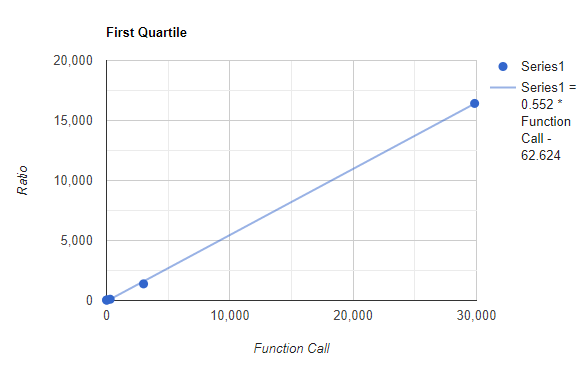
\includegraphics[width=.85\textwidth]{hfd1.PNG} % scale 75%
\end{figure}

    \begin{figure}[H]
	\centering
	\caption{Third Quartile}
	\label{fig:Third Quartile}
	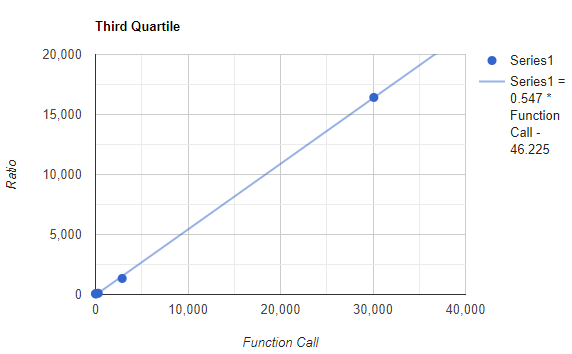
\includegraphics[width=.85\textwidth]{hfd2.PNG} % scale 75%
\end{figure}

\newpage

    \begin{figure}[H]
	\centering
	\caption{Max}
	\label{fig:Max}
	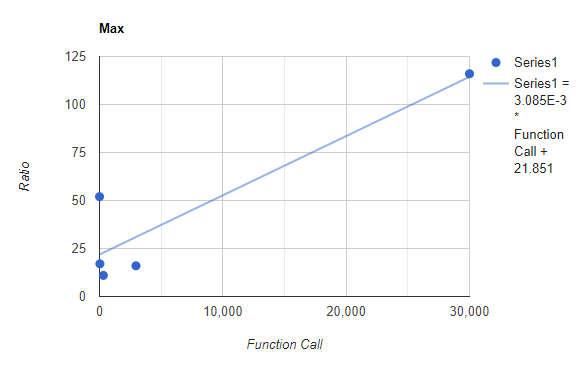
\includegraphics[width=.85\textwidth]{hfd3.PNG} % scale 75%
\end{figure}

    \begin{figure}[H]
	\centering
	\caption{Min}
	\label{fig:Min}
	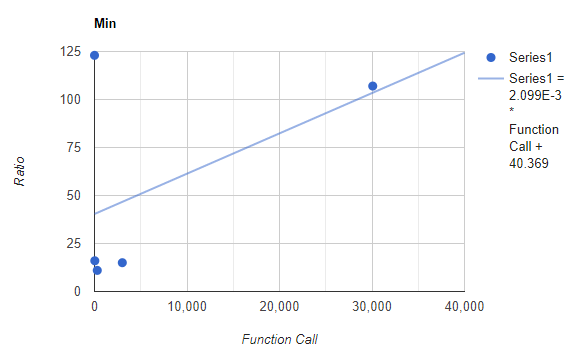
\includegraphics[width=.85\textwidth]{hfd4.PNG} % scale 75%
\end{figure}
\newpage

    \begin{figure}[H]
	\centering
	\caption{Mean}
	\label{fig:Mean}
	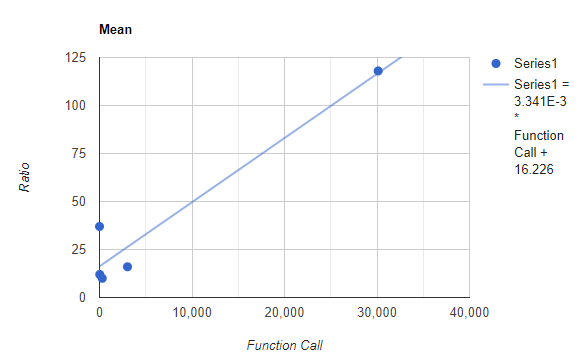
\includegraphics[width=.85\textwidth]{hfd5.PNG} % scale 75%
\end{figure}

    \begin{figure}[H]
	\centering
	\caption{Standard Deviation}
	\label{fig:Standard Deviation}
	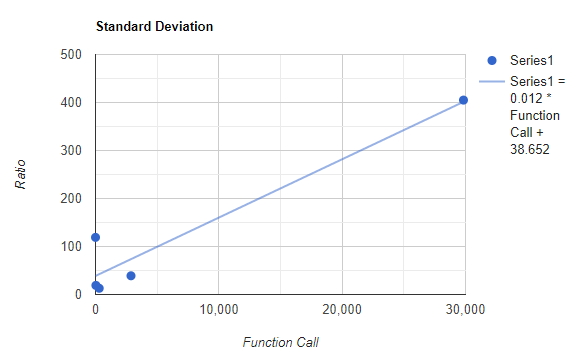
\includegraphics[width=.85\textwidth]{hfd6.PNG} % scale 75%
\end{figure}
\newpage

    \begin{figure}[H]
	\centering
	\caption{Median}
	\label{fig:Median}
	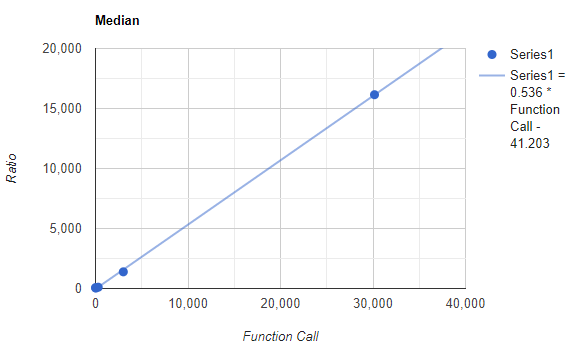
\includegraphics[width=.85\textwidth]{hfd7.PNG} % scale 75%
\end{figure}

All of the graphs are really look like linear lines because the quantities are huge and in the very small parts it changes qucikly , for example in 10 datas sample , it is quite quick but when working with 100000 datas sample the computation cost and time is large

\section{Sliding Window}

Sliding Window is a simple algorithm to one way system can move towards in a kernel size. For example we have ten input stream and we have a windows size 3, starting from a selected position window will 
start to progress the stream by sliding the window . With this approach we will have the first 3 elements and when we slide one step we will have 2,3,4 elements.

    For this homework,  We can assume there is 10 element array . Window will start from 0 index and ends at a special position F. We take K minimum elements  among all F elements and store them in a max heap. When we created the first max-heap we will move forward one step ahead. Heap will be updated.After that again window will slide one step but this time heap will not be updated. Updating the max-heap only depends on the windows neew elements relation with the removed element of window. This procedure will continue until all the heap is processed and the selected size of max-heap will be found.
    Complexity analysis of this algorithm, worst case complexity of sliding window algorithm would be O(N^2 * K). K is included as it takes O(K) complexity to build a heap of K elements.
\end{document}

